
\appendix

\chapter{Pflichtenheft}
%\addcontentsline{toc}{chapter}{Anhang A Pflichtenheft}
\label{Pflichtenheft}

Das Pflichtenheft wurde während der Einarbeitung des Projekts erstellt und Herr Jensen vorgelegt. Es bestimmt einerseits den Umfang der Arbeit mit entsprechenden Erläuterungen.


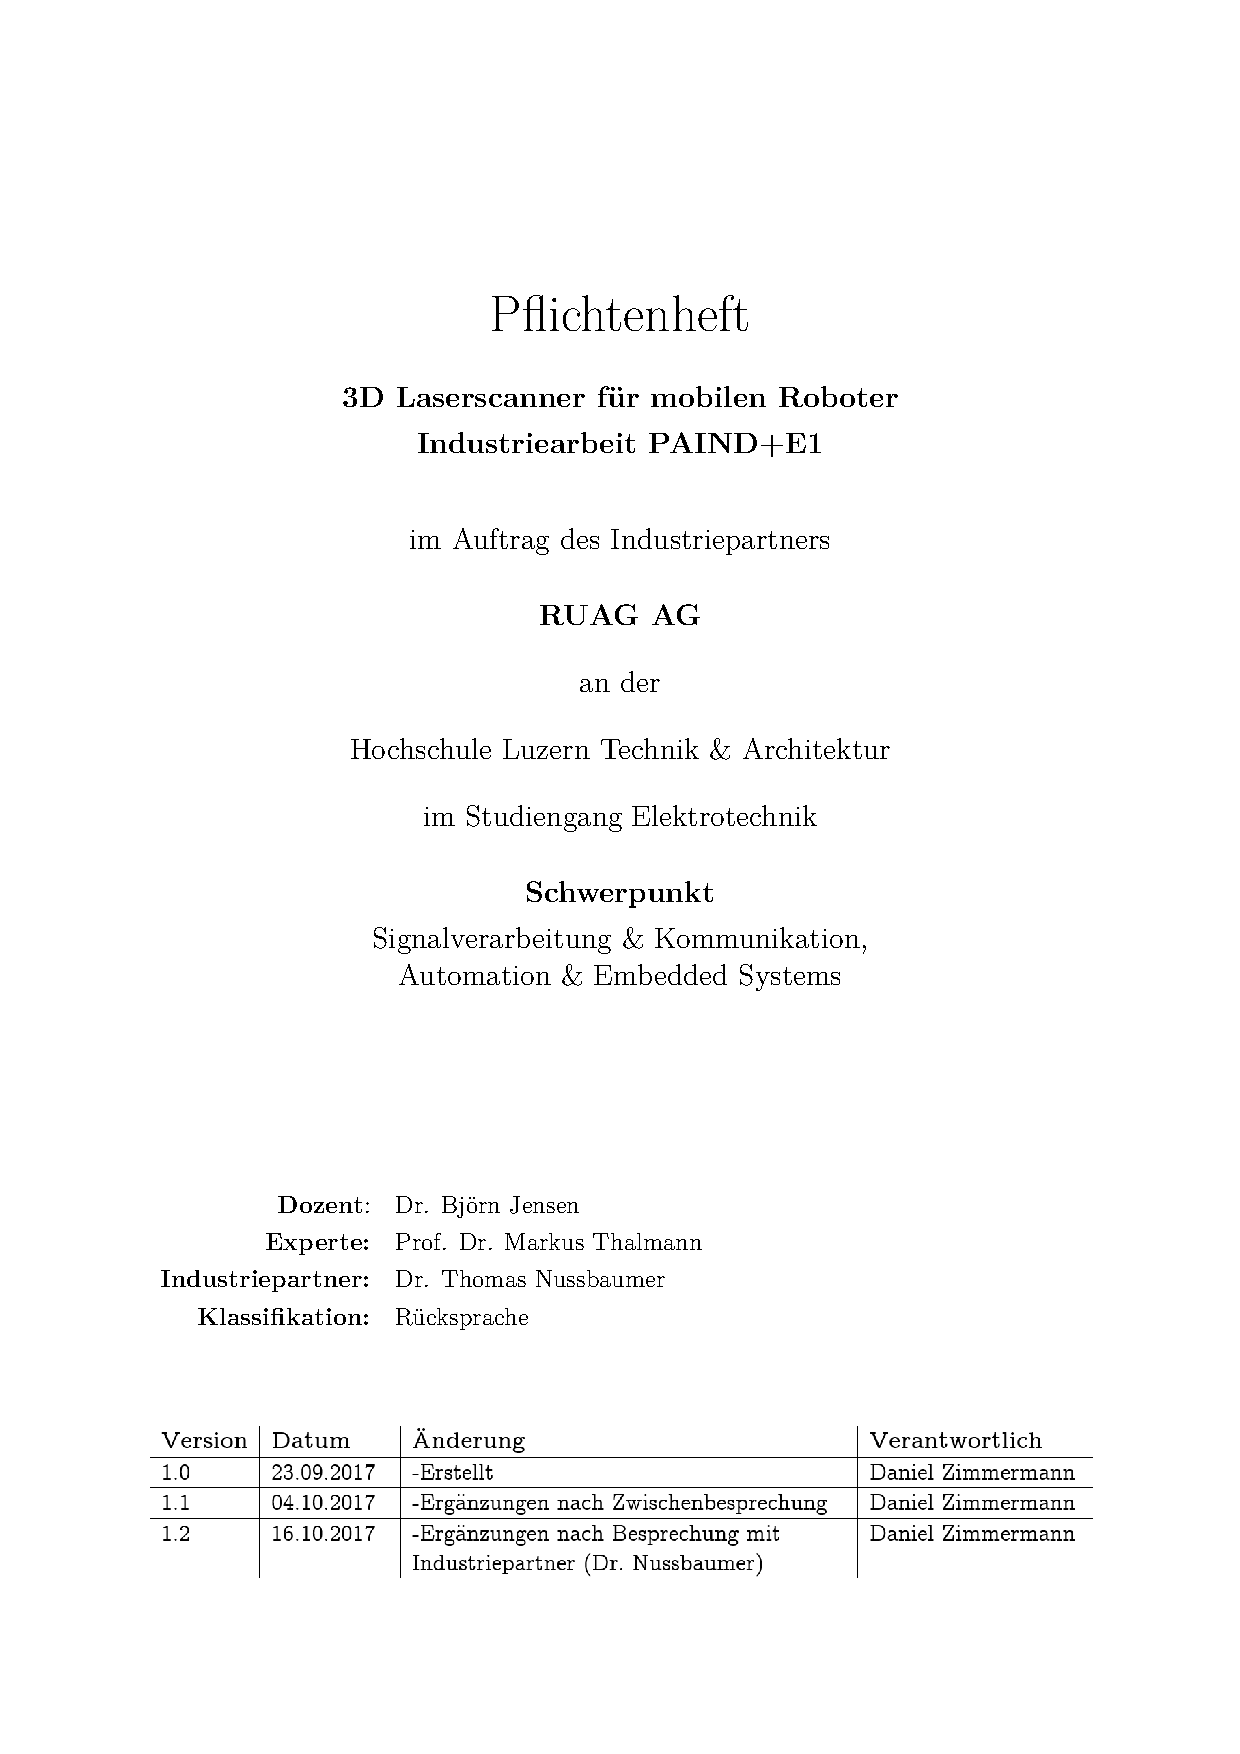
\includepdf[pages ={1-9}]{chapters/Pflichtenheft_V1_2.pdf}



\chapter{Projektmanagment}
%\addcontentsline{toc}{chapter}{Anhang B Projektmanagment}
\label{Projektmanagment}

Auf den nachfolgenden Seite ist ein detaillierter Projektplan einsehbar. Die Projektphasen sind dabei übergeordnet und dienen als Meilensteine. Weitere Meilensteine sind entsprechend markiert. Die Projektphasen wurden im Pflichtenheft Anhang A erläutert und geben Auskunft über den Umfang der Phase. Im detaillierten Projektplan sind für die jeweiligen Arbeitspakete entsprechende zeitliche Soll-/Istwerte in Stunden [h] angegeben. Diese sollen Auskunft geben, welche Arbeitspakete ungenügend eingeschätzt wurden. Bedeutende Aufwandsabweichungen werden im Kapitel \ref{chap:Reflektion} erklärt.

	\clearpage
\KOMAoptions{paper=A3,paper=landscape,pagesize}
\recalctypearea
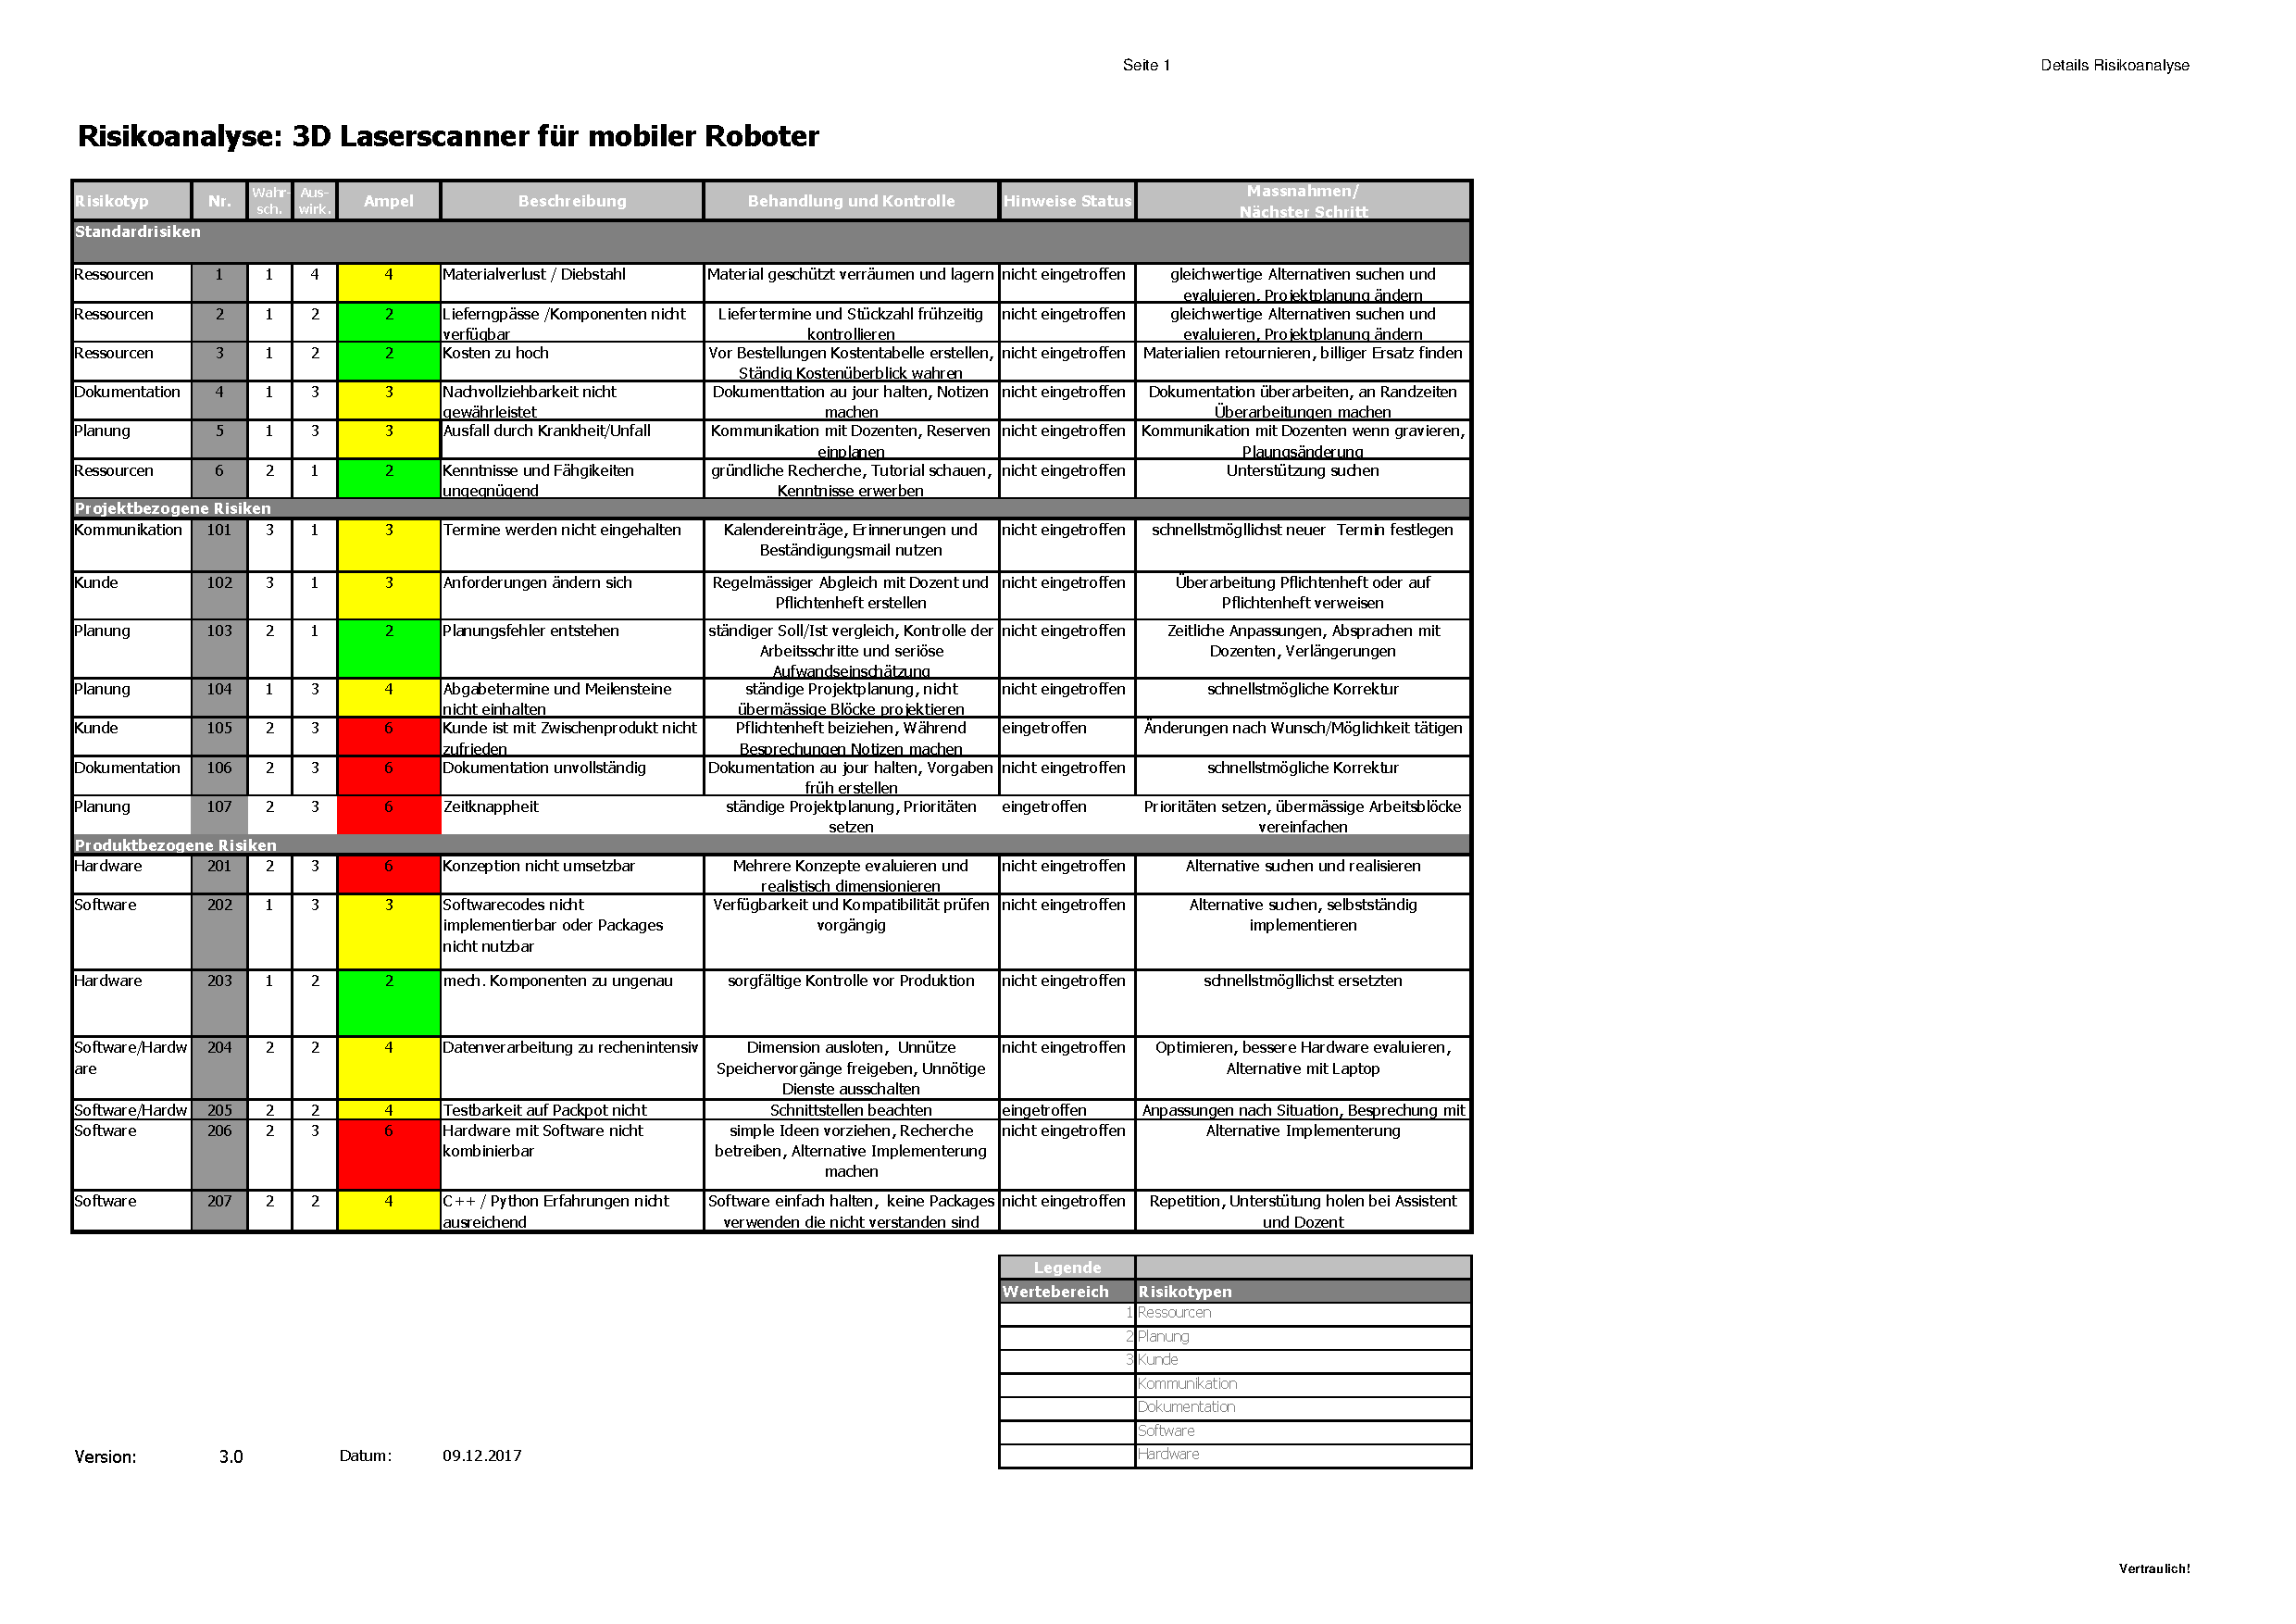
\includepdf[noautoscale]{chapters/Risikoanalyse_V2.pdf}
\clearpage
\KOMAoptions{paper=A4,paper=portrait, pagesize}
\recalctypearea

\chapter{Risikoanalyse}

	\clearpage
	\KOMAoptions{paper=A3,paper=landscape,pagesize}
	\recalctypearea
		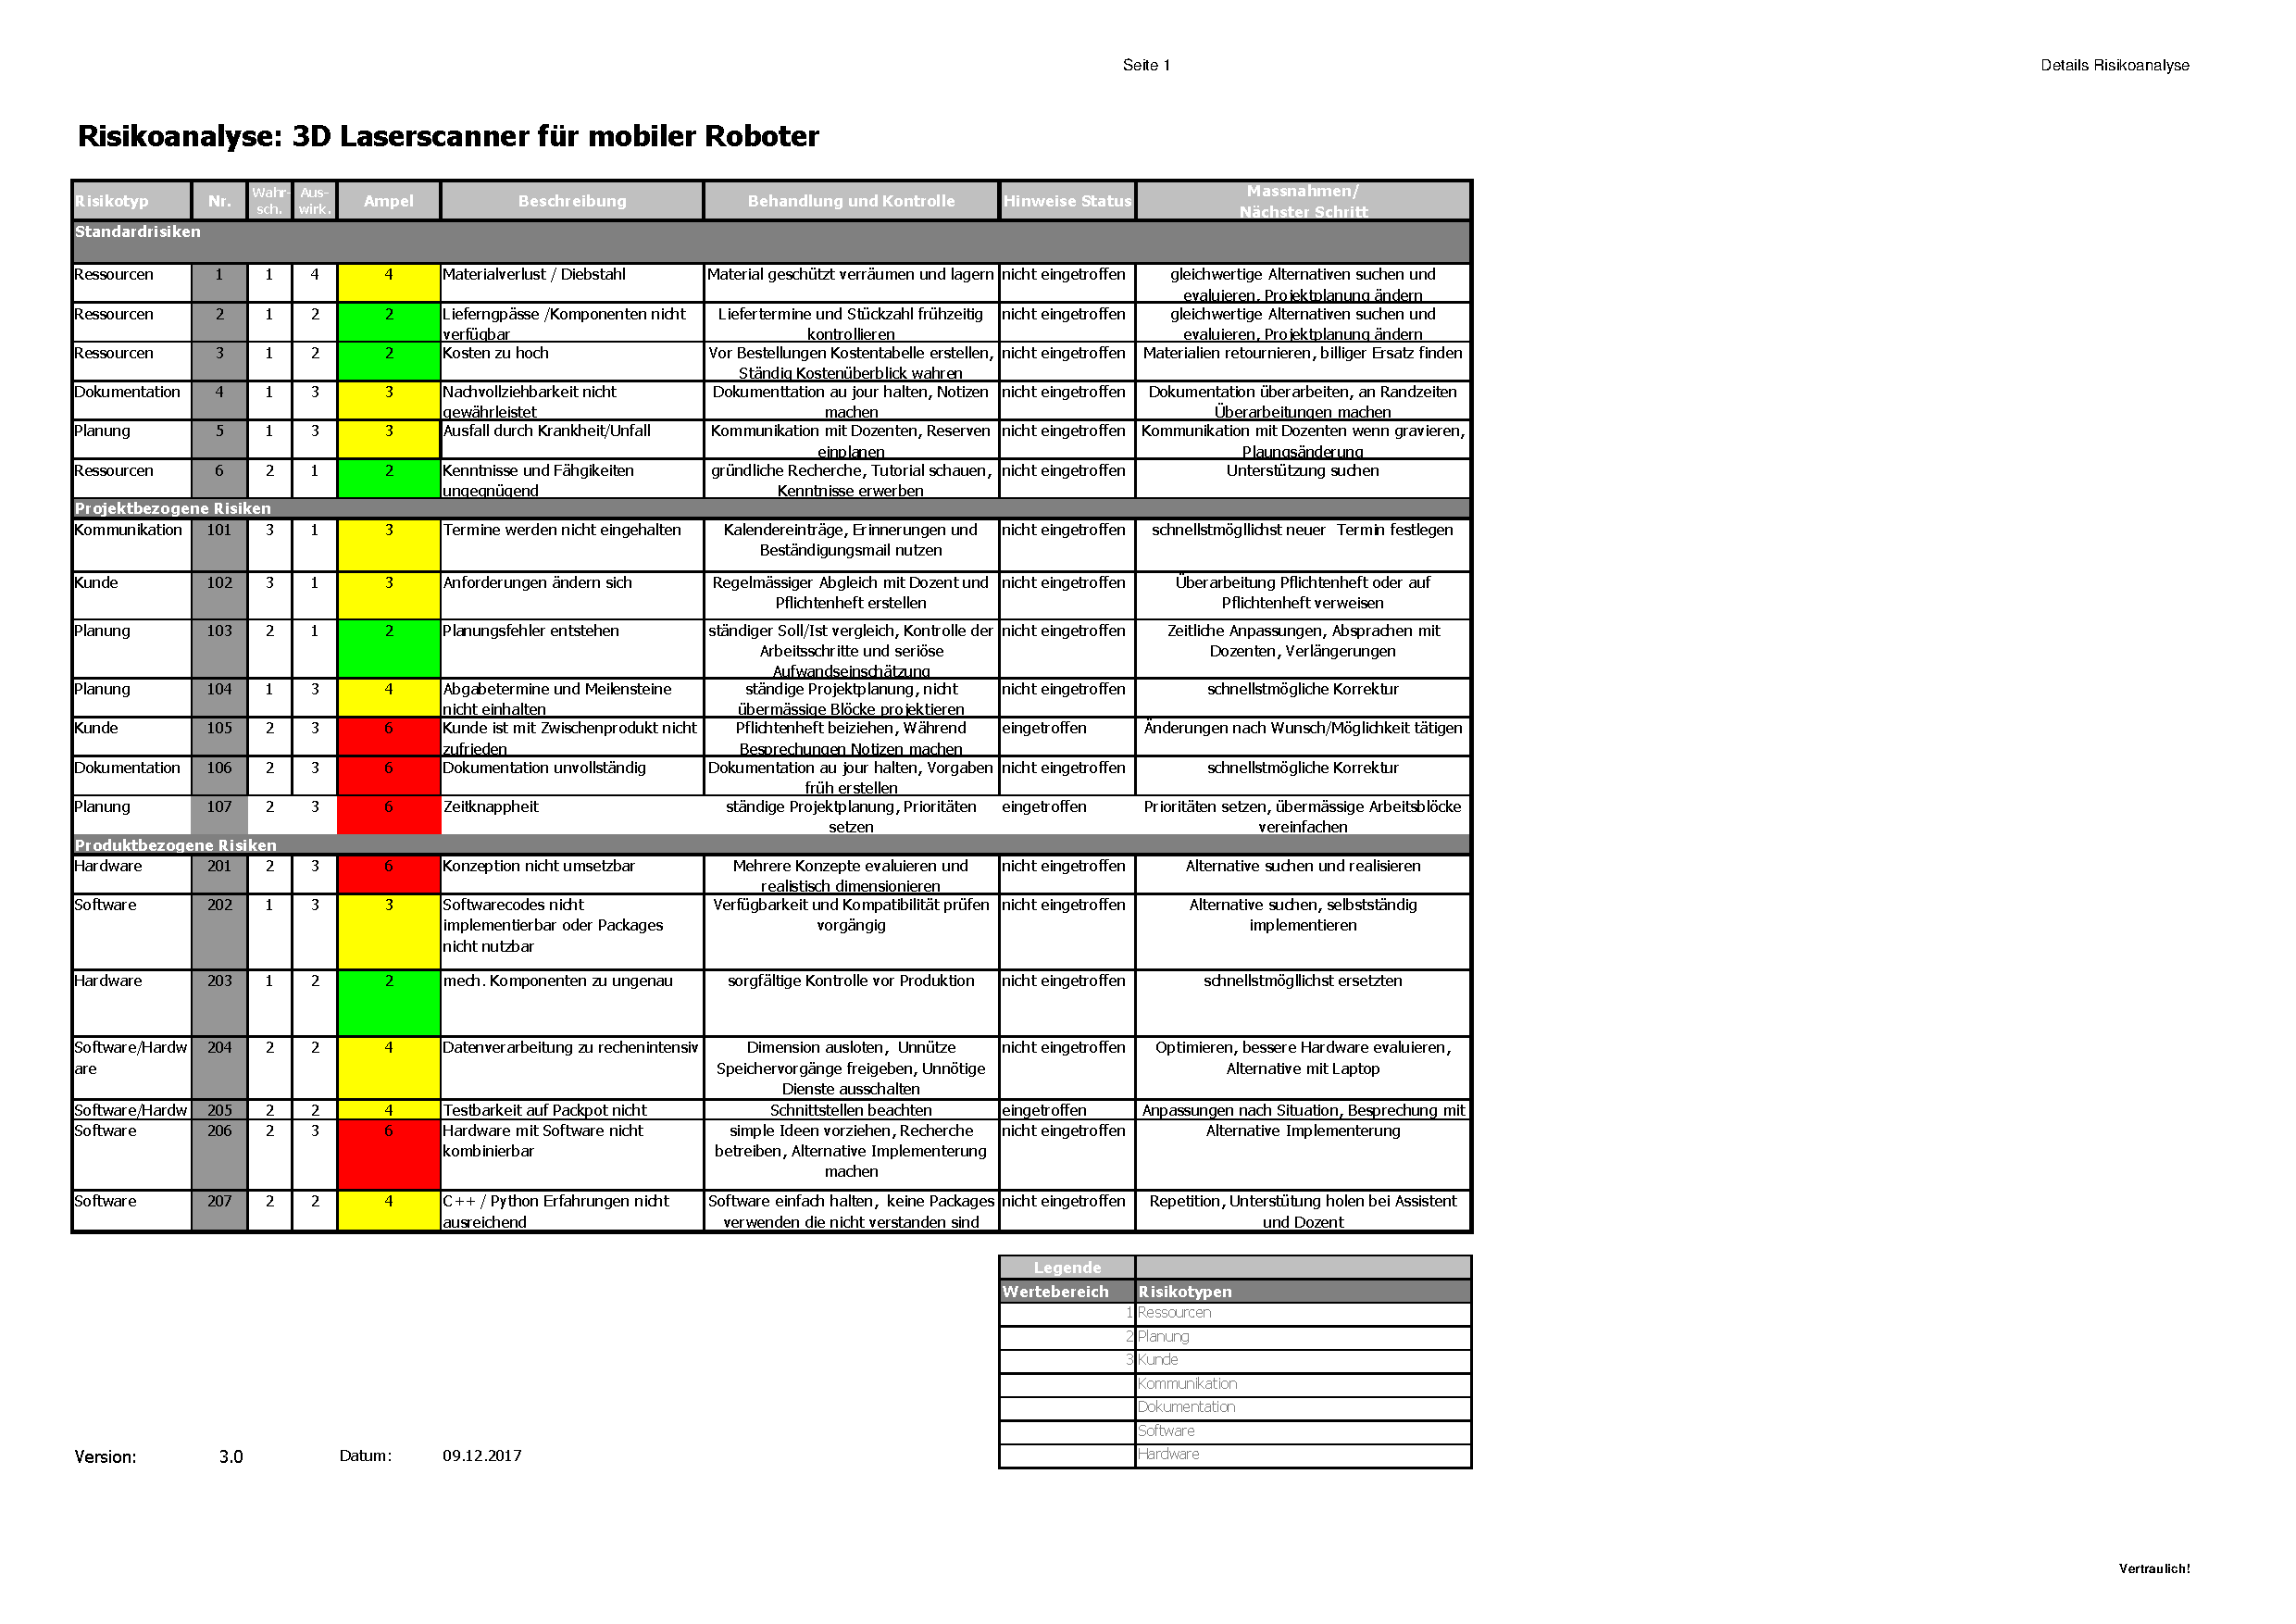
\includepdf[noautoscale]{chapters/Risikoanalyse_V2.pdf}
	\clearpage
	\KOMAoptions{paper=A4,paper=portrait, pagesize}
	\recalctypearea

\chapter{Aufgabenstellung}

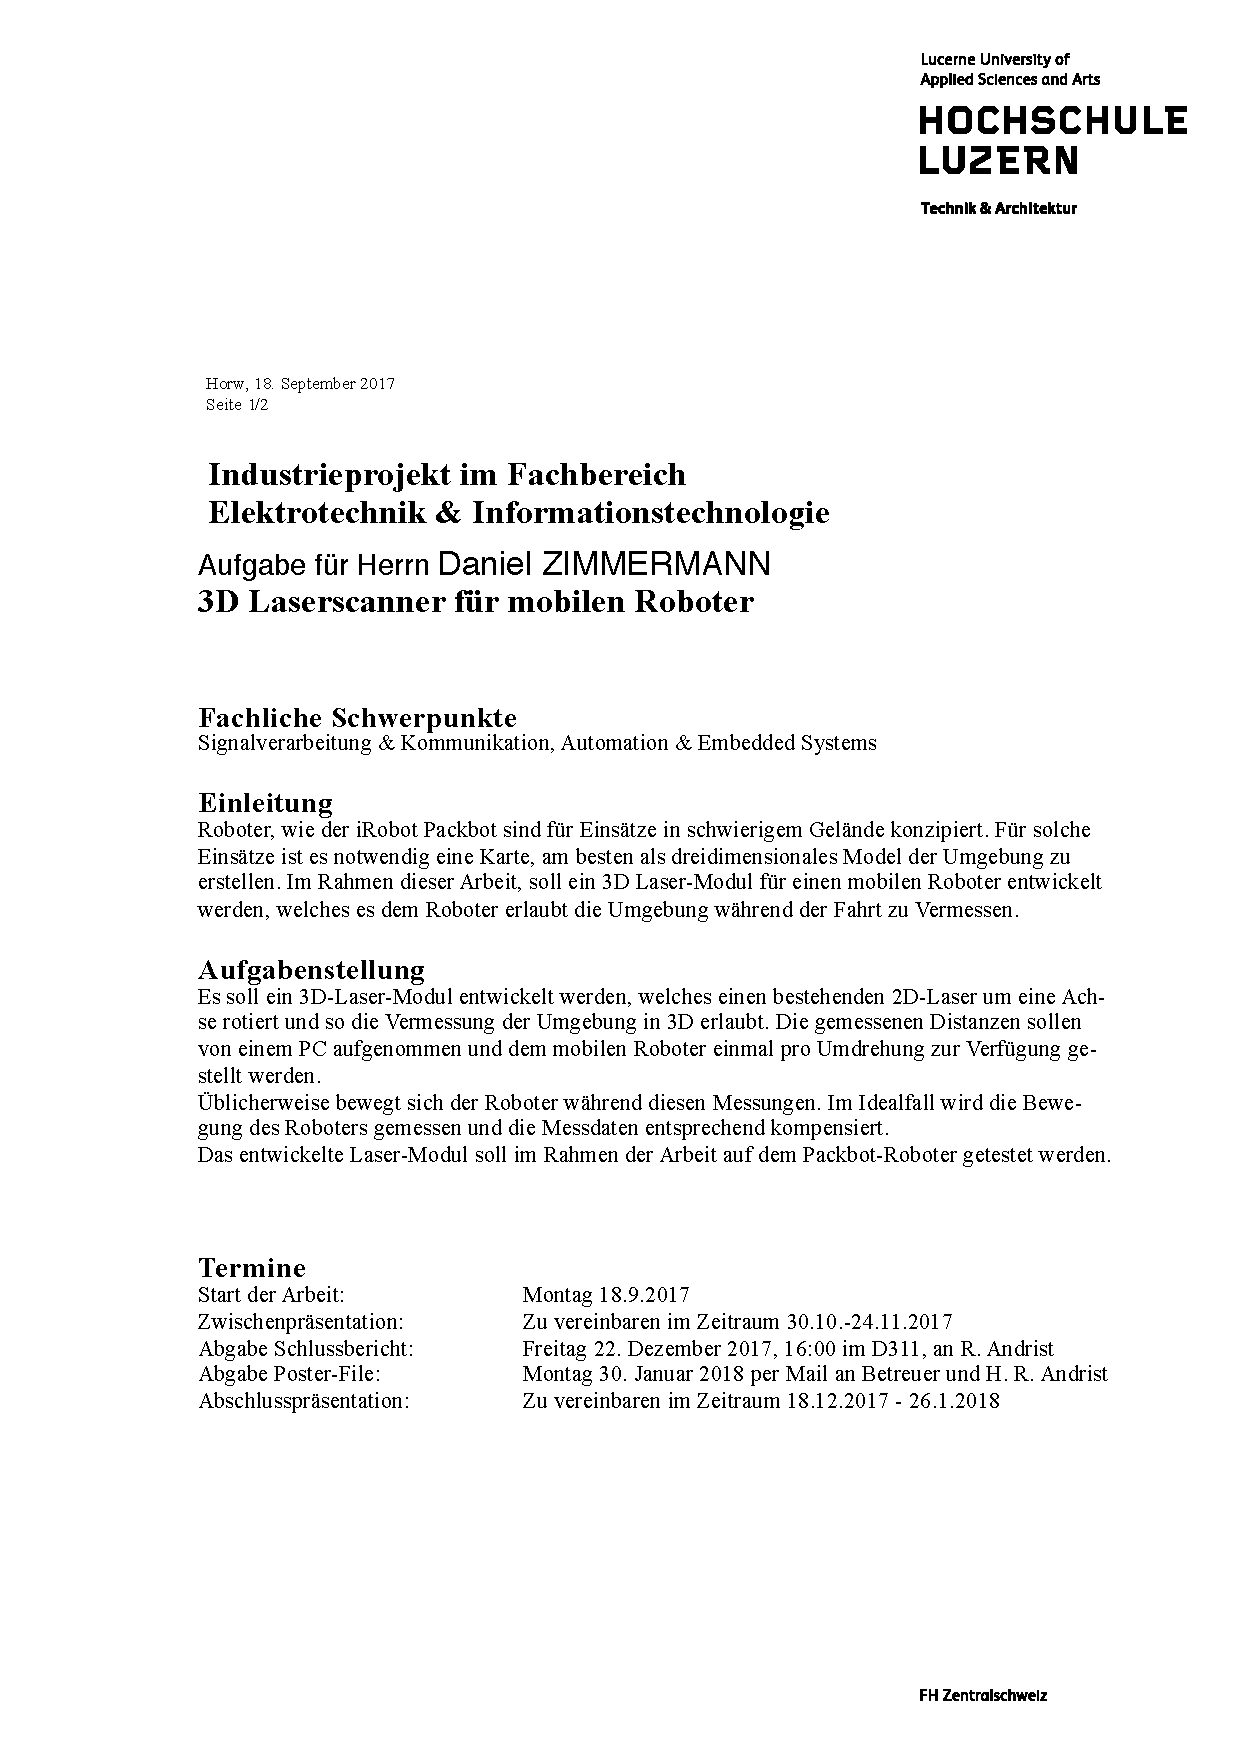
\includepdf{chapters/Aufgabenstellung.pdf}
